Upon the recent shift of application architectures from monolithic to containers and micro-services, serverless computing has risen as a promising cloud provider offering where applications and services are composed by event-driven functions. It represents an revolutionary programming and deployment paradigm known as Function as a Service (FaaS). Using serverless model, developers can easily build up applications in a cloud without concerning server provisioning at the infrastructure level. Those functions are usually programmed in high-level languages and triggered by events either from external source or, more often, internal cloud services. Thus, serverless architecture allows the application to distribute across the cloud by providing function-level abstraction.

Moreover, this function-level abstraction does not only abstract away the infrastructure management work from developers, but also, more importantly, provides more fine-grained computational resource isolation and usage, meaning each serverless function can autoscale independently based on the scale of incoming events. Providing such elasticity effectively avoid the single point failure and bottleneck service in a data-intensive application. From this perspective, serverless architecture is an ideal system for machine learning applications, especially for online training~\cite{ref:online} and model serving, because they usually transfer and handle large amount of data, but the volume of each batch is uncertain and highly volatile depending on the data generation in that period. The flexibility that serverless functions deliver perfectly address such issue via event-driven mechanism. 

To enable such event-driven system, one concerning situation is that those machine learning applications usually evolve heterogeneous IoT devices, ranging from temperature sensors to mobile phones to autonomous drones, which are the primary data sources in the physical world. If the applications execute, at least partially, on the edge cloud, it could save lengthy round-trip time of transmitting data and make the application infinitely close to real-time. Our work is motivated by such demand and explores the effectiveness and efficiency of executing machine learning applications on the edge cloud. 

An immediate difficulty we face is the scarcity of computational resources on edge cloud relative to high-demanding machine learning applications. In addition, no cloud provider offers serverless function that leverages accelerator like GPU. In our work, we construct a hybrid cloud system that enables serverless function to utilize GPU, which substantially accelerates the execution of machine learning applications. We consider it as one of the key contributions of our research.

\begin{figure}
    \centering
    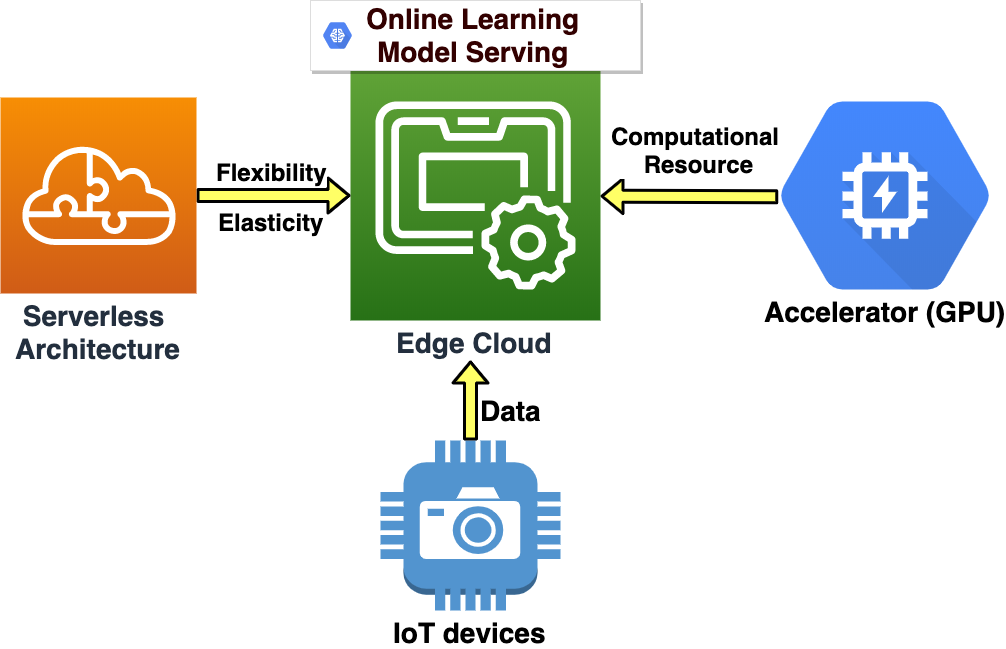
\includegraphics[scale=0.25]{figures/edge}
    \caption{The Design Principle of STOIC }
    \label{fig:edge}
\end{figure}

Figure~\ref{fig:edge} illustrates the design principal of our proposed system, STOIC (Serverless TeleOperable Hybrid Cloud). In our design, the center edge cloud is supported by three underpinnings: IoT devices stream data in batches for training and inference; serverless architecture provides flexibility and elasticity to handle auto-scaling and unbalanced data payload; accelerator offers additional computational resource for extra large dataset and compute-intensive machine learning applications. In this paper, we discuss the design and implementation of this architecture, investigate the efficacy and evaluate its performance empirically. We found STOIC reduces total response time, ranging from 6.48\% to 32.05\%, comparing with four single runtimes. Finally, we show both related and future work and conclude.
